\section{Workstations}
All workstations run \href{http://www.debian.org/}{Debian} stable, version 8,
codename \href{https://www.debian.org/releases/jessie/}{Jessie}.

\subsection{Graphical User Interface (GUI) Applications}

\subsection{\href{http://christian.amsuess.com/tools/arandr/}{ARandR}}
ARandR allows you to configure a second monitor.

\begin{figure}[h!]
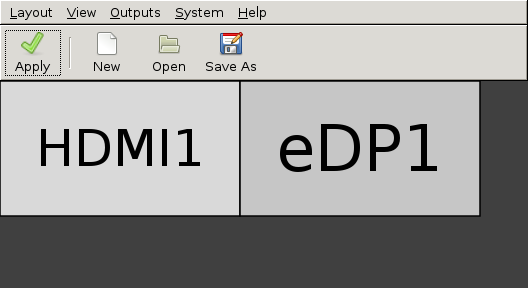
\includegraphics[keepaspectratio=true,height=1.10\textheight,width=1.00\textwidth,angle=0]{screen-arandr.png}
 \caption{ARandR, configure second monitor}
 \label{fig:screen-arandr}
\end{figure}

\subsection{\href{http://www.arduino.cc}{Arduino}}

Arduino is a series of free hardware controller boards and free software
development tools. The software application ``Arduino'' is used to compile
firmware for LulzBot 3D printers. The controller board used in LulzBots is
derived from Arduino hardware.

\begin{figure}[h!]
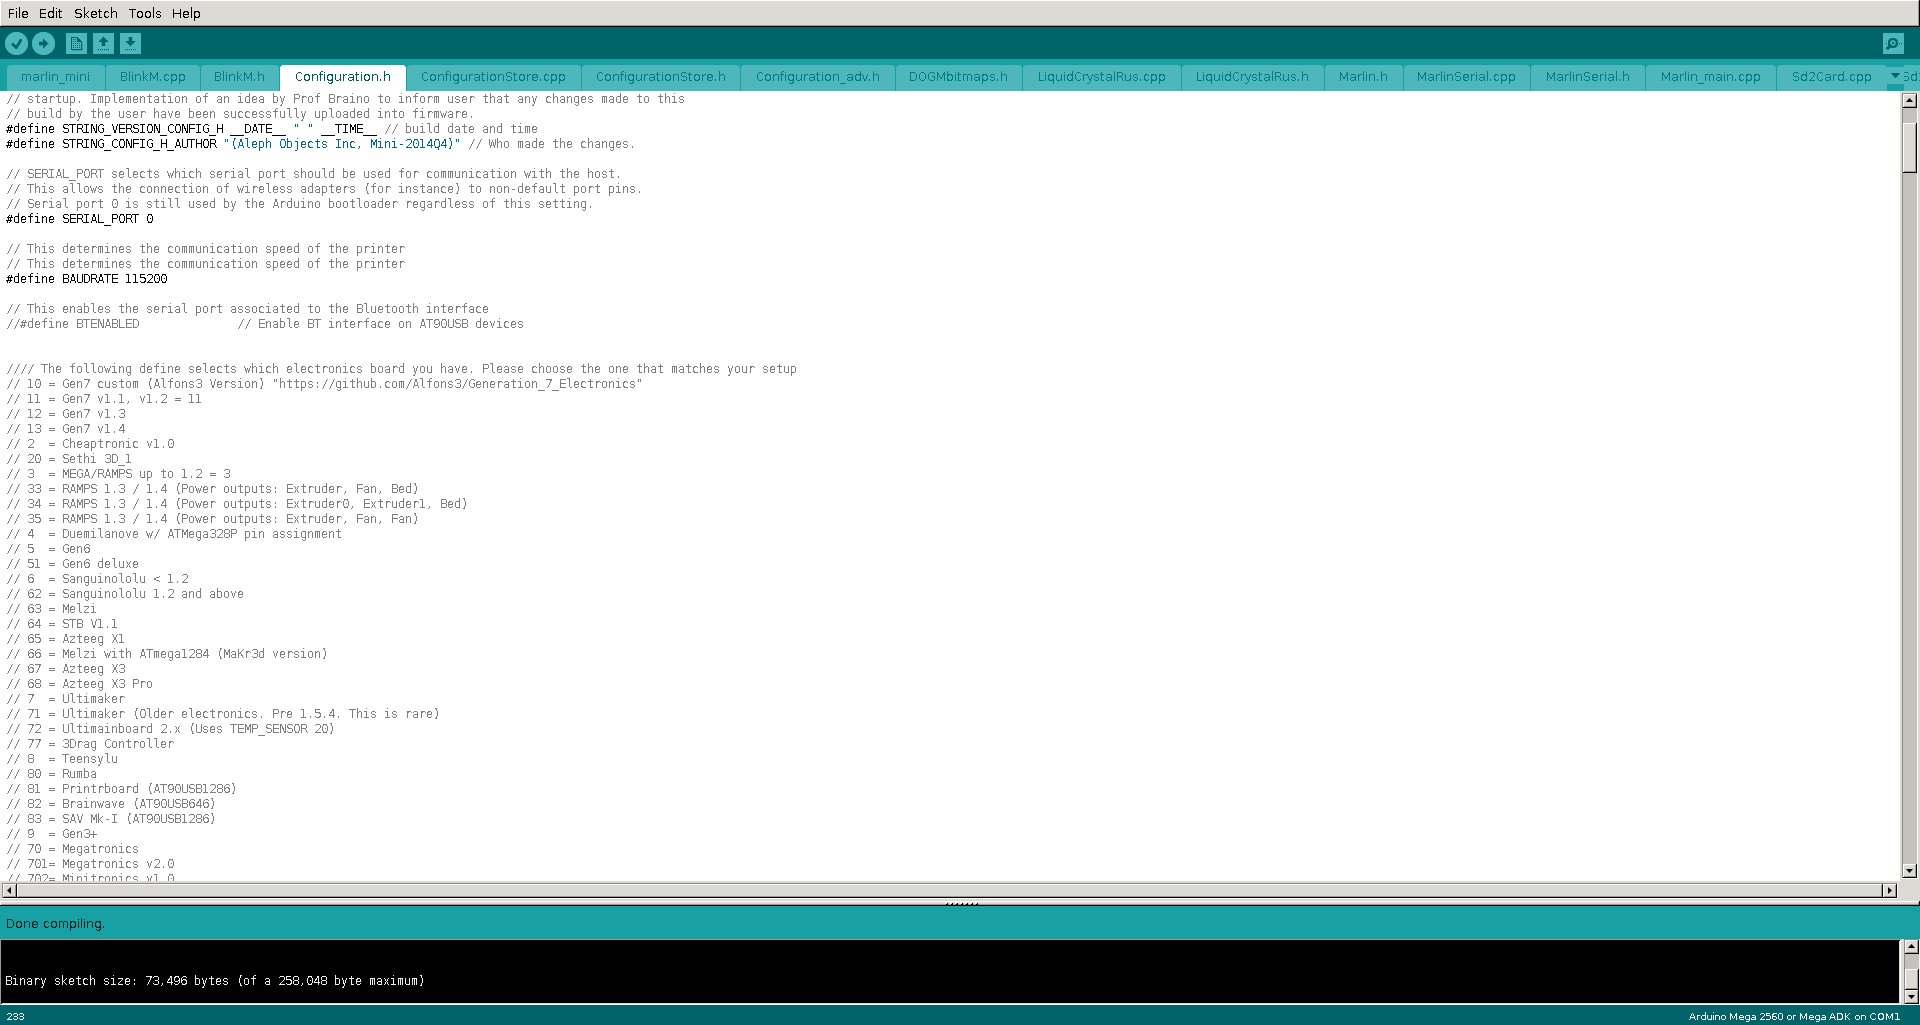
\includegraphics[keepaspectratio=true,height=1.10\textheight,width=1.00\textwidth,angle=0]{screen-arduino.png}
 \caption{Arduino, compile LulzBot 3D printer firmware}
 \label{fig:screen-arduino}
\end{figure}

\subsection{\href{http://audacity.sourceforge.net/}{Audacity}}

 Audacity is a multi-track audio editor for GNU/Linux.
 It is designed for easy recording, playing and editing of
 digital audio.  Audacity features digital effects and spectrum
 analysis tools.  Editing is very fast and provides unlimited
 undo/redo.
 
 Supported file formats include Ogg Vorbis, WAV, AIFF, and AU.

\begin{figure}[h!]
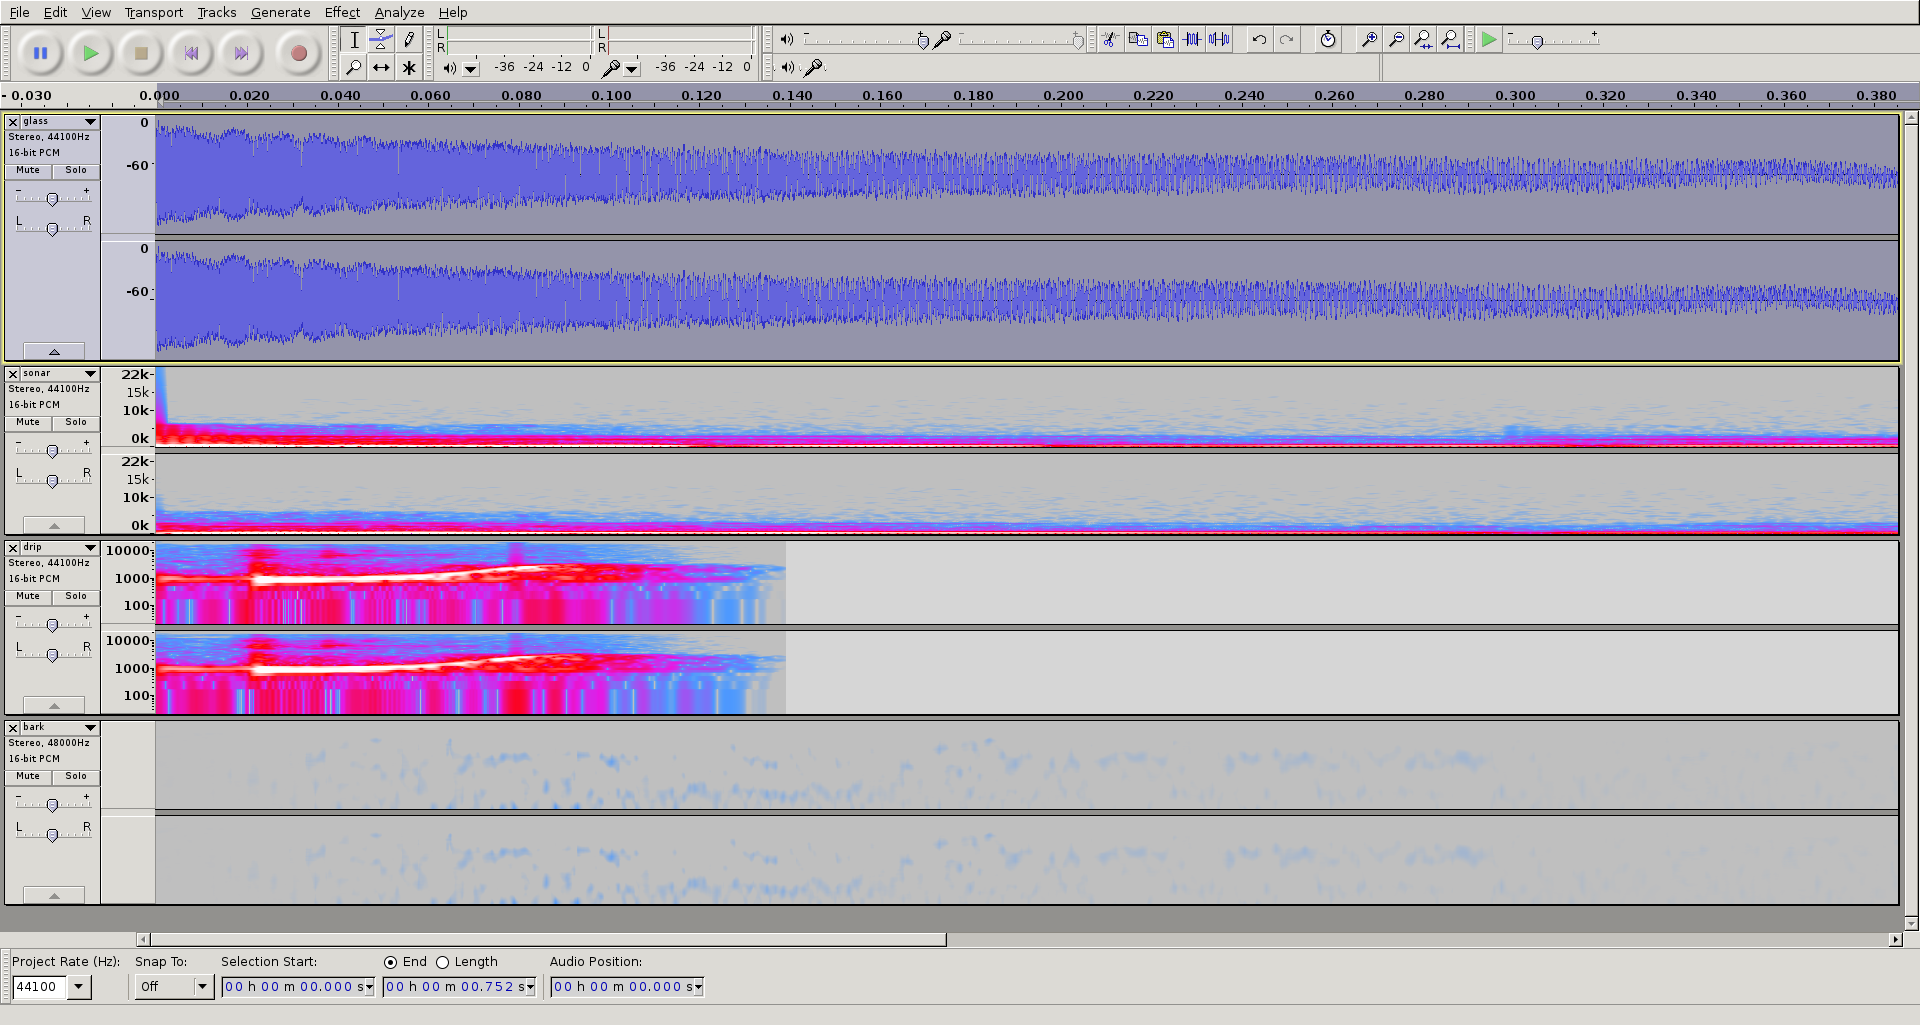
\includegraphics[keepaspectratio=true,height=1.10\textheight,width=1.00\textwidth,angle=0]{screen-audacity.png}
 \caption{Audacity audio editor}
 \label{fig:screen-audacity}
\end{figure}

\subsection{\href{http://www.blender.org/}{Blender}}

Blender is a 3D CAD application that can be used to make 3D printable objects.

 Blender is an integrated 3d suite for modelling, animation, rendering,
 post-production, interactive creation and playback (games).

\begin{figure}[h!]
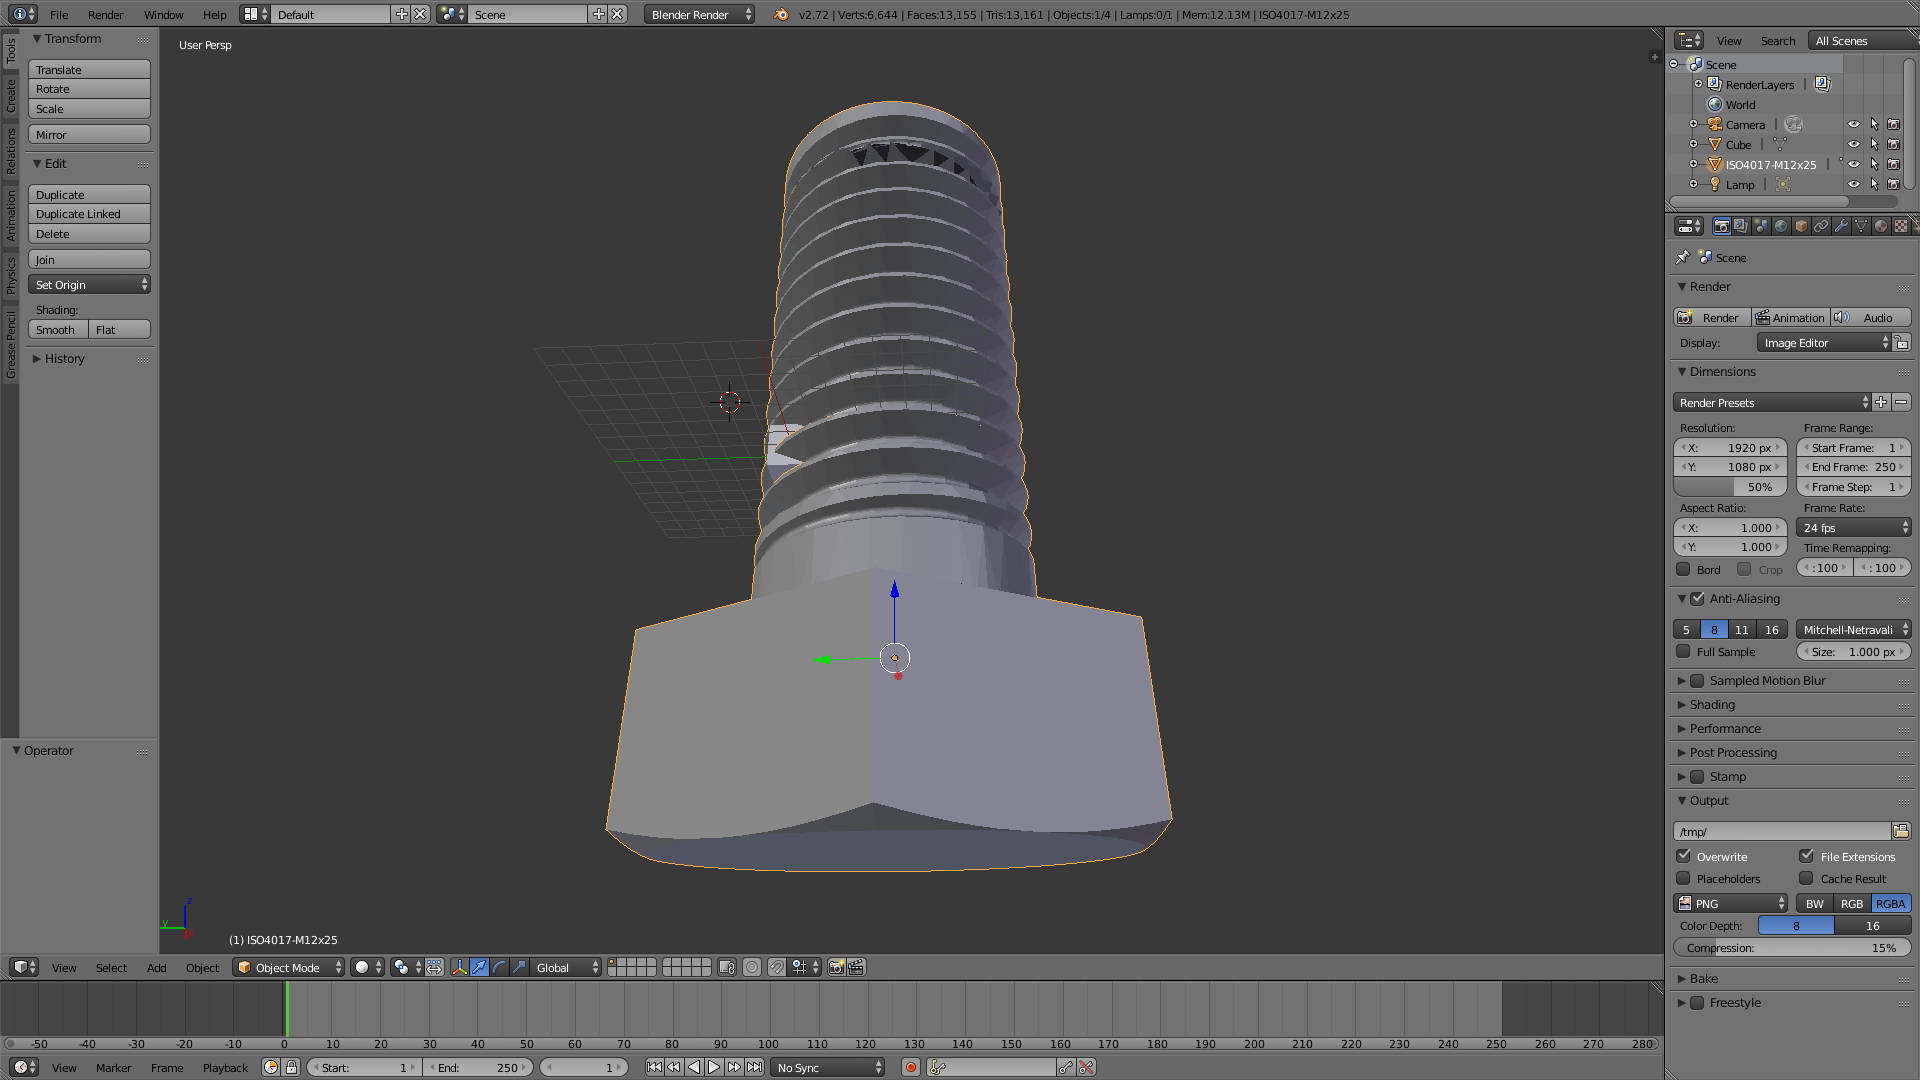
\includegraphics[keepaspectratio=true,height=1.10\textheight,width=1.00\textwidth,angle=0]{screen-blender.png}
 \caption{Blender 3D CAD}
 \label{fig:screen-blender}
\end{figure}

\subsection{\href{http://www.chromium.org/Home}{Chromium}}

 Web browser that aims to build a safer, faster, and more stable internet
 browsing experience.
 
\begin{figure}[h!]
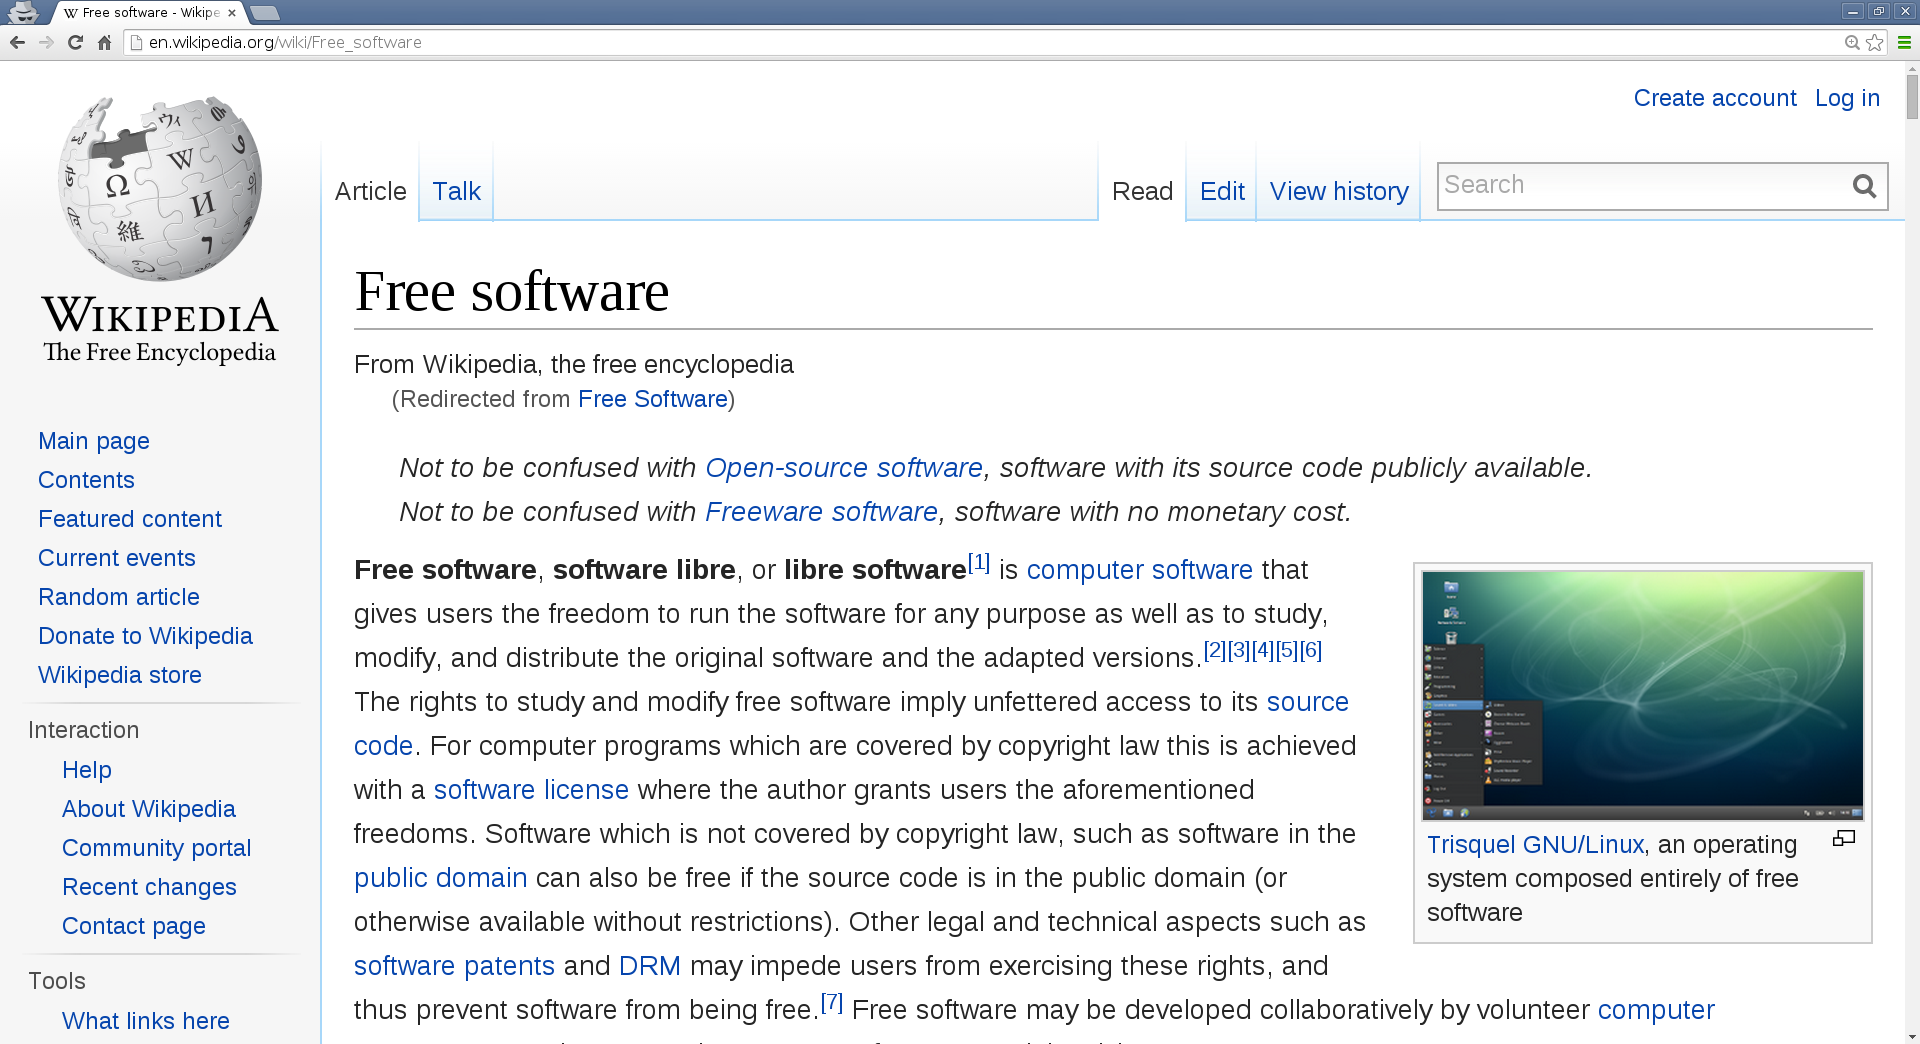
\includegraphics[keepaspectratio=true,height=1.10\textheight,width=1.00\textwidth,angle=0]{screen-chromium.png}
 \caption{Chromium web browser viewing Wikipedia}
 \label{fig:screen-chromium}
\end{figure}

\subsection{\href{http://github.com/alephobjects/Cura}{LulzBot Cura}}

LulzBot Cura is the main slicer and 3D printer control software for LulzBot 3D
printers.

\begin{figure}[h!]
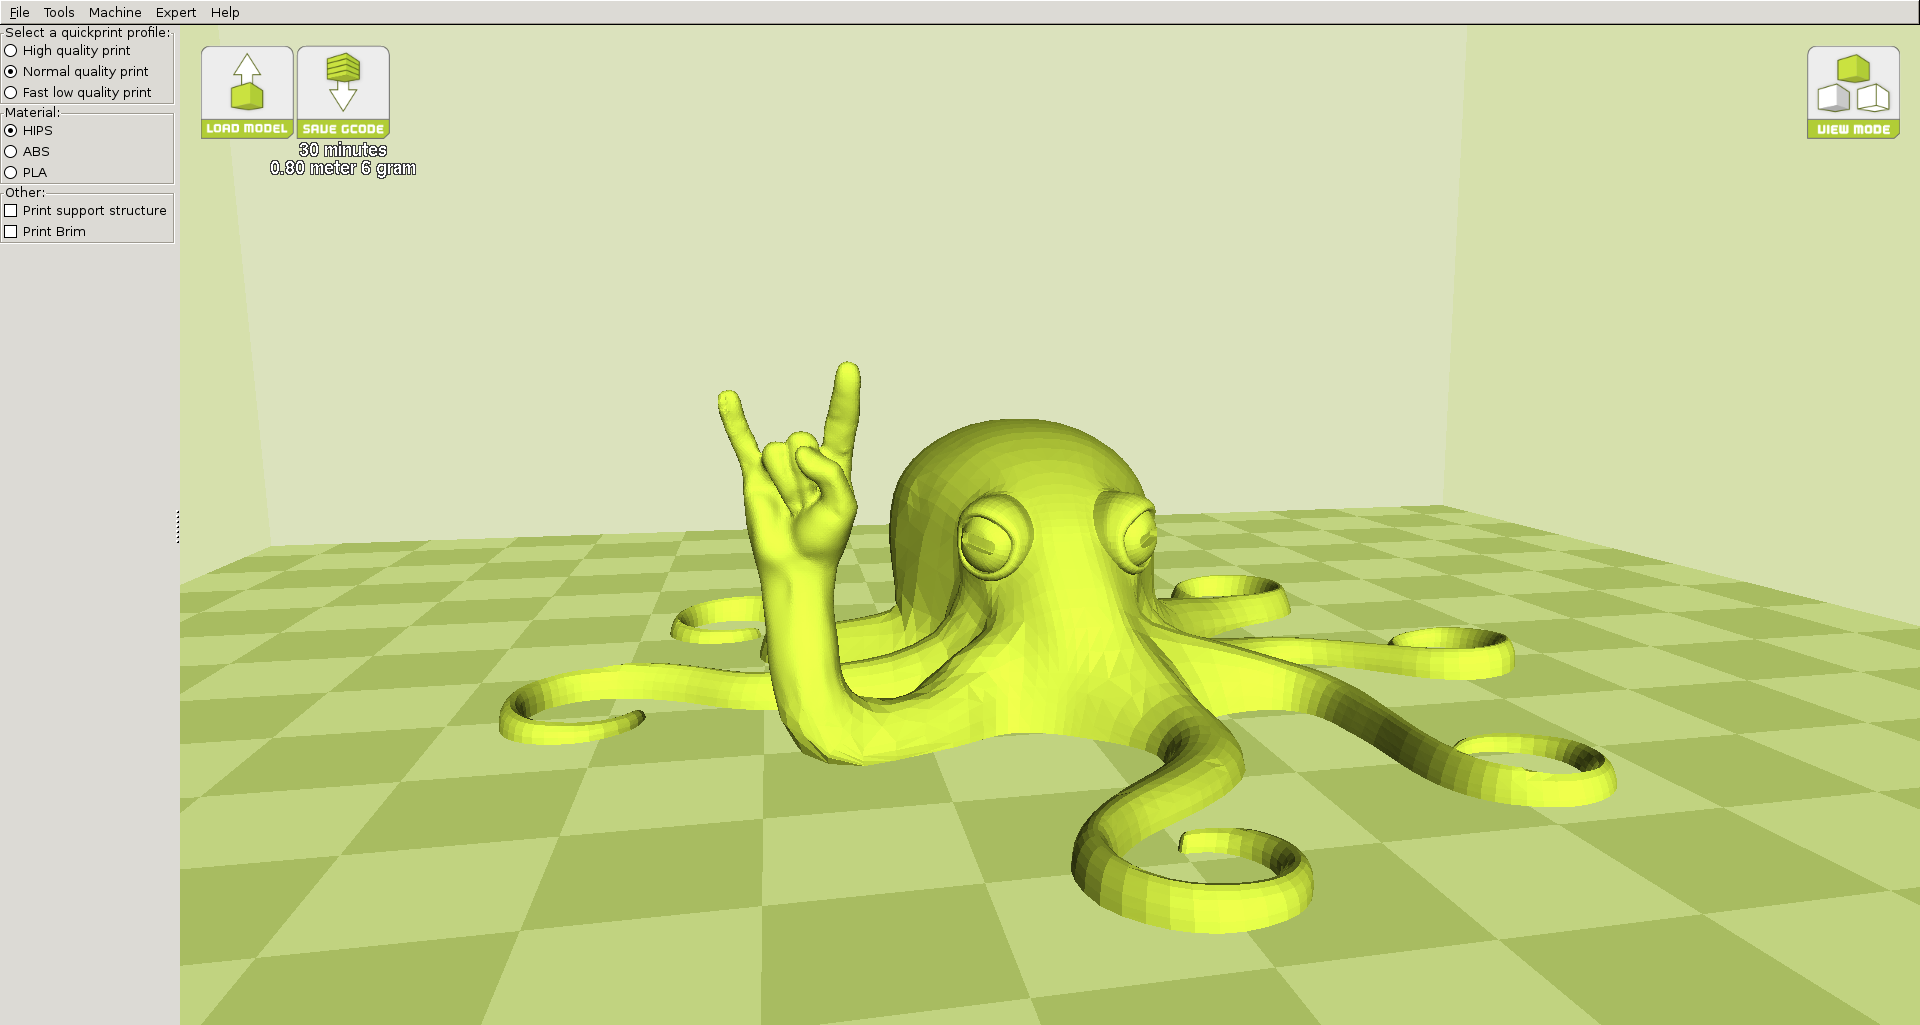
\includegraphics[keepaspectratio=true,height=1.10\textheight,width=1.00\textwidth,angle=0]{screen-lulzbot-cura.png}
 \caption{LulzBot Cura 3D printer control software}
 \label{fig:screen-lulzbot-cura}
\end{figure}

%\subsection{\href{http://www.darktable.org/}{Darktable}}
%
% Darktable manages your digital negatives in a database and lets you view
% them  through a zoomable lighttable. It also enables you to develop raw
% images and enhance them.
% 
%\subsection{\href{http://live.gnome.org/Dia}{Dia}}
%
% Dia is an editor for diagrams, graphs, charts etc. There is support for UML
% static structure diagrams (class diagrams), Entity-Relationship diagrams,
% network diagrams and much more. Diagrams can be exported to postscript and
% many other formats.

\subsection{\href{https://wiki.gnome.org/Apps/Web}{Epiphany}}

 Epiphany is a simple yet powerful web browser targeted at
 non-technical users. Its principles are simplicity and standards
 compliance.
 
\begin{figure}[h!]
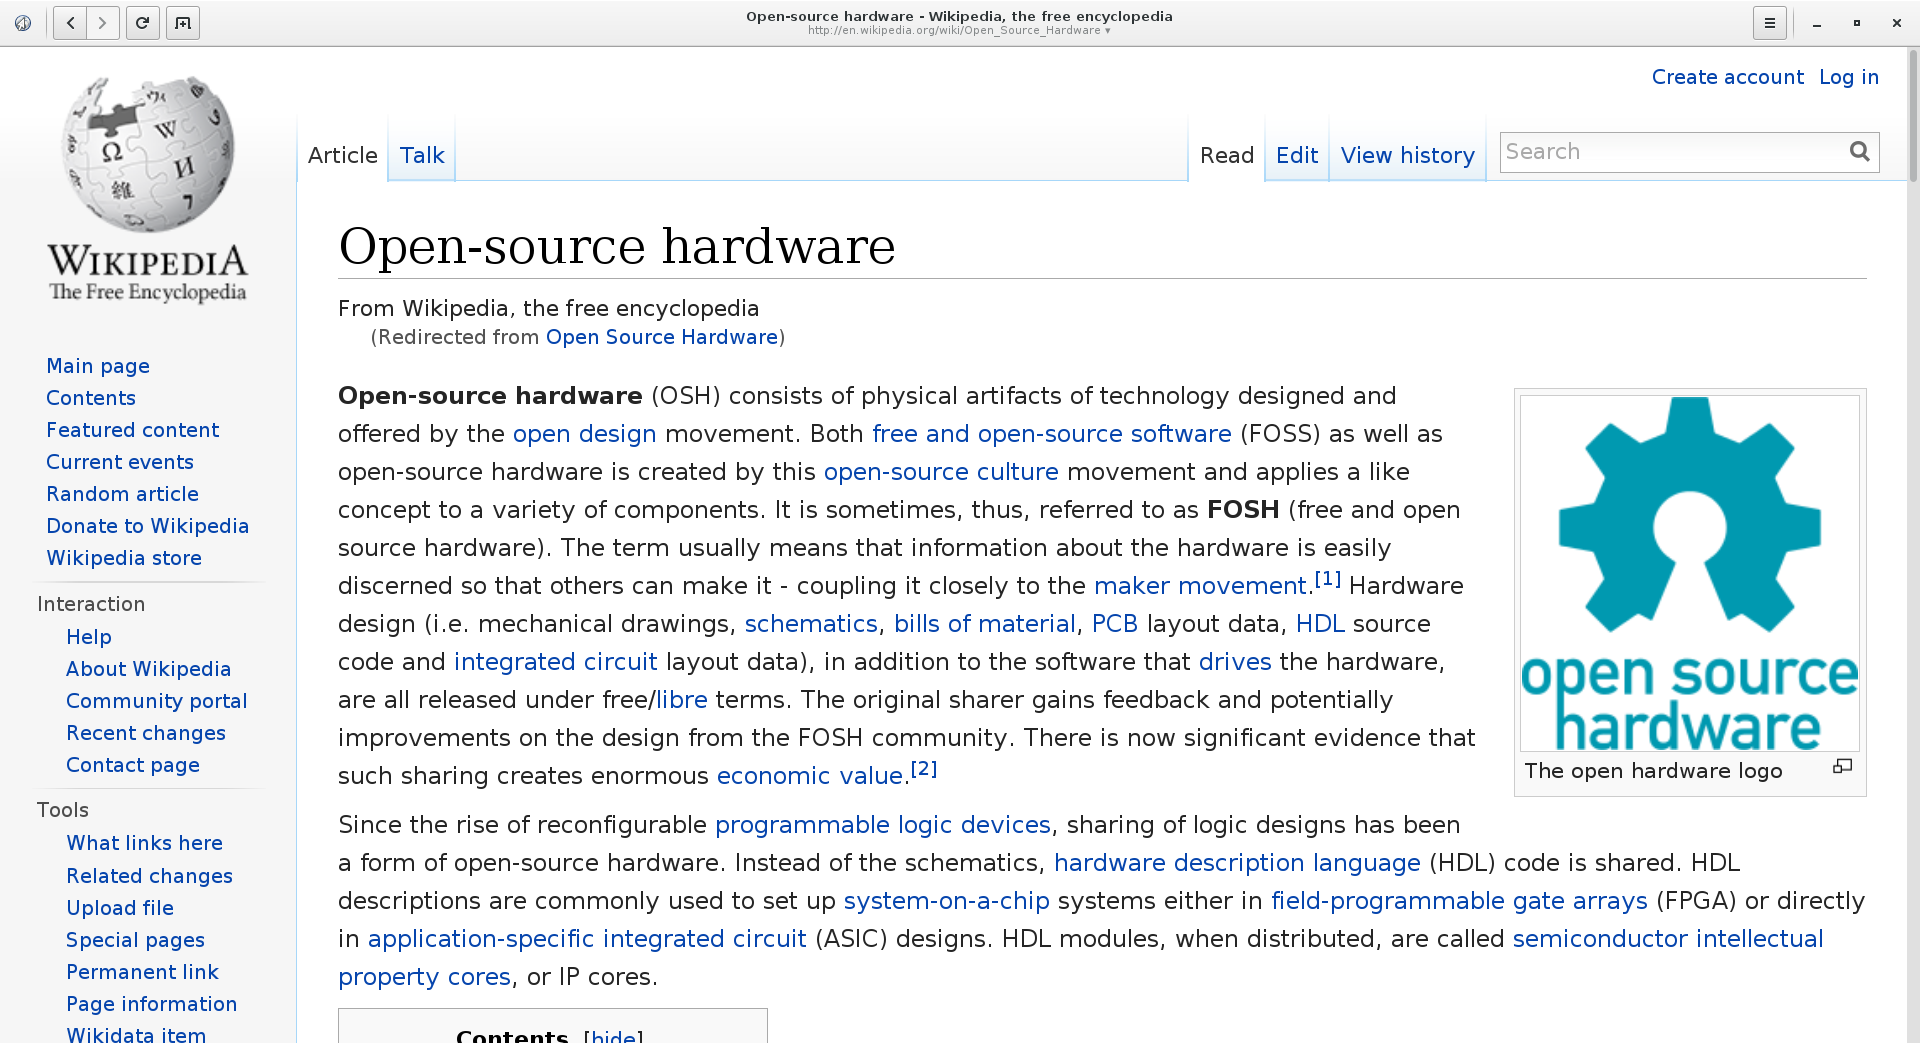
\includegraphics[keepaspectratio=true,height=1.10\textheight,width=1.00\textwidth,angle=0]{screen-epiphany.png}
 \caption{Epiphany web browser viewing Wikipedia}
 \label{fig:screen-epiphany}
\end{figure}

\subsection{\href{https://wiki.gnome.org/Apps/Evince}{Evince}}

 Evince is a simple multi-page document viewer.  It can display and print
 PostScript (PS), Encapsulated PostScript (EPS), DjVu, DVI, Portable
 Document Format (PDF) and XML Paper Specification (XPS) files.
 When supported by the document, it also allows searching for text,
 copying text to the clipboard, hypertext navigation, and
 table-of-contents bookmarks.

\begin{figure}[h!]
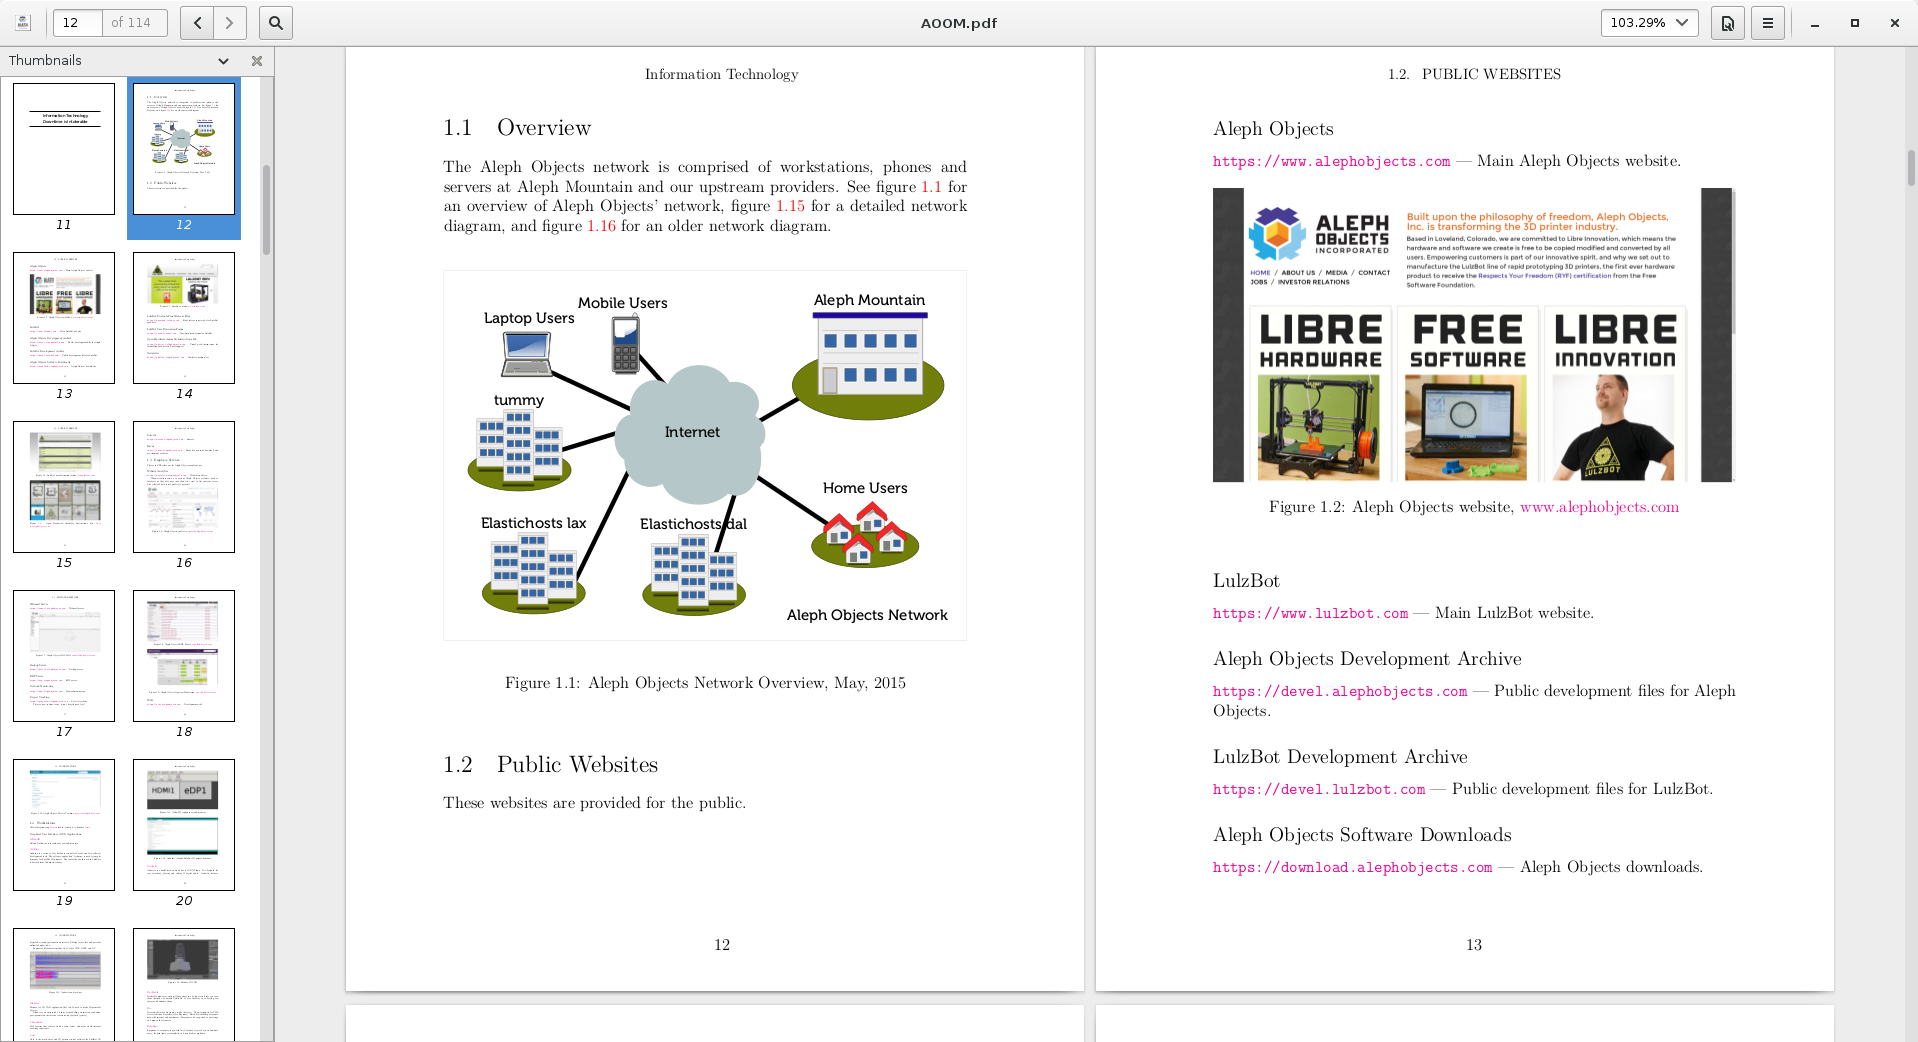
\includegraphics[keepaspectratio=true,height=1.10\textheight,width=1.00\textwidth,angle=0]{screen-evince.png}
 \caption{Evince PDF viewer viewing AOOM}
 \label{fig:screen-evince}
\end{figure}

\subsection{\href{http://fileroller.sourceforge.net/}{File-Roller}}

 File-roller is an archive manager. It allows you to:

\begin{itemize}
 \item Create and modify archives.
 \item View the content of an archive.
 \item View a file contained in an archive.
 \item Extract files from the archive.
\end{itemize}
 
 File-roller supports the following formats:

\begin{itemize}
 \item Tar (.tar) archives, including those compressed with
    gzip (.tar.gz, tgz), bzip (.tar.bz, tbz), bzip2 (.tar.bz2, tbz2),
    compress (.tar.Z, taz), lzip (.tar.lz, tlz), lzop (.tar.lzo, tzo),
    lzma (.tar.lzma) and xz (.tar.xz)
 \item Zip archives (.zip)
 \item Jar archives (.jar, ear, war)
 \item 7z archives (.7z)
 \item iso9660 CD images (.iso)
 \item Lha archives (.lzh)
 \item Archiver archives (.ar)
 \item Comic book archives (.cbz)
 \item Single files compressed with gzip (.gz), bzip (.bz), bzip2 (.bz2),
    compress (.Z), lzip (.lz), lzop (.lzo), lzma (.lzma) and xz (.xz)
\end{itemize}
 
 File-roller can extract following formats:

\begin{itemize}
 \item Cabinet archives (.cab)
 \item Debian binary packages (.deb)
 \item Xar archives (.xar)
\end{itemize}
 
 File-roller doesn't perform archive operations by itself, but relies on
 standard tools for this.

\subsection{\href{http://freecadweb.org/}{FreeCAD}}

FreeCAD is a 3D CAD application.
It can make objects suitable for 3D printing. It is used to design many
parts on LulzBot 3D printers.

\begin{figure}[h!]
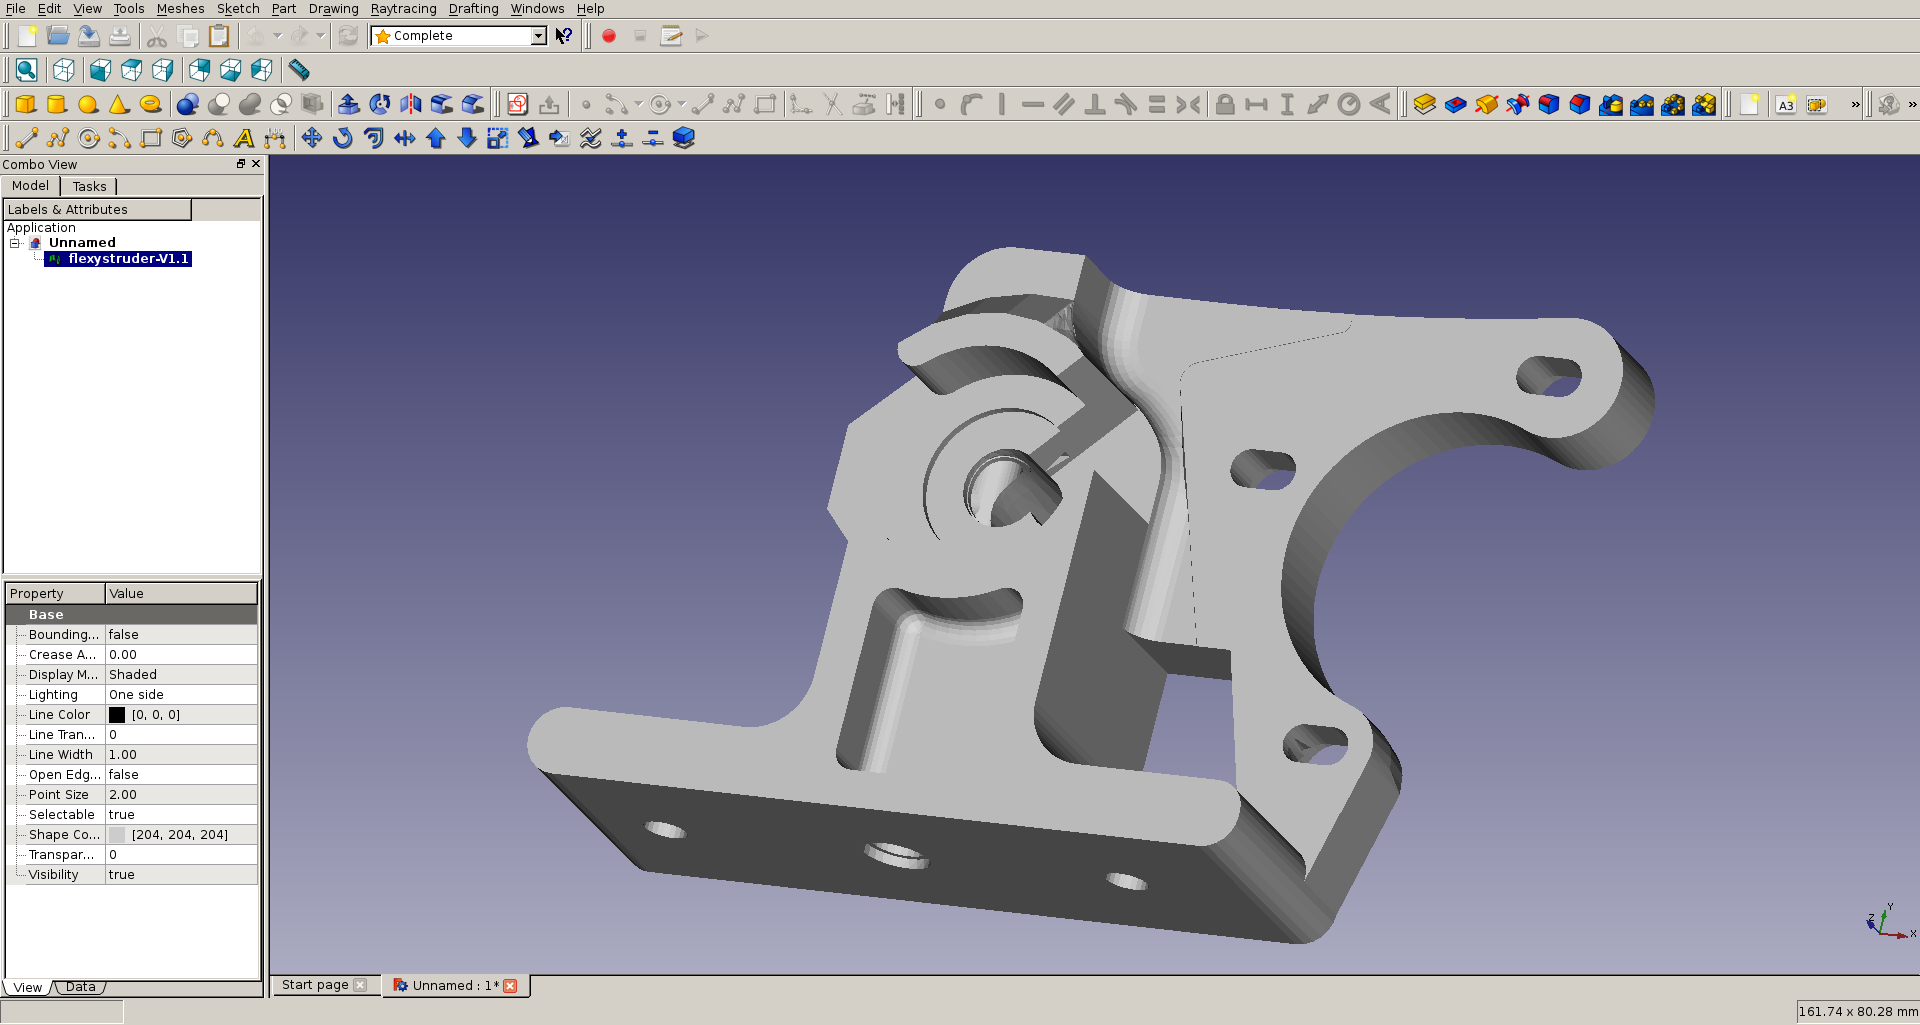
\includegraphics[keepaspectratio=true,height=1.10\textheight,width=1.00\textwidth,angle=0]{screen-freecad.png}
 \caption{FreeCAD}
 \label{fig:screen-freecad}
\end{figure}

\subsection{\href{http://galculator.sourceforge.net/}{Galculator}}

 Galculator is a calculator.

\begin{figure}[h!]
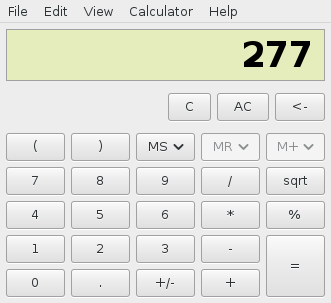
\includegraphics[keepaspectratio=true,height=0.50\textheight,width=0.50\textwidth,angle=0]{screen-galculator.png}
 \caption{Galculator}
 \label{fig:screen-galculator}
\end{figure}

\subsection{\href{https://wiki.gnome.org/Apps/Gedit}{Gedit}}

 gedit is a text editor which supports most standard editor features,
 extending this basic functionality with other features.
 
 Its core feature set includes syntax
 highlighting of source code, auto indentation and printing and print preview
 support.
 
\subsection{\href{http://geeqie.sourceforge.net/}{Geeqie}}

 Geeqie is a browser for graphics files offering single click viewing.
 It includes thumbnail view, zoom, filtering
 features, and external editor support.

\subsection{\href{http://www.gimp.org/}{GIMP}}

 GIMP is an advanced picture editor. You can use it to edit, enhance, and
 retouch photos and scans, create drawings, and make your own images.
 It has a large collection of professional-level editing tools and
 filters. Numerous
 fine-control settings and features like layers, paths, masks, and
 scripting give you total control over your images.
 
\subsection{\href{http://glabels.sourceforge.net/}{gLabels}}

 gLabels is a lightweight program for creating labels, barcodes, business
 cards and media covers. It is designed to
 work with various laser/ink-jet peel-off label and business card sheets that
 you'll find at most office supply stores.
 
 gLabels also supports mail merge from sources such as CSV files, vCards.

\subsection{\href{https://git.gnome.org/browse/gnome-color-manager}{GNOME Color Manager}}

 GNOME Color Manager is a set of graphical utilities for color
 management.

\subsection{\href{}{GNOME Screenshot}}
Screenshots can also be taken thusly, and by default will be written to the
\texttt{Pictures} directory.

\begin{enumerate}
 \item\texttt{ALT-F2} --- to bring up a command dialog in the middle of the screen
 \item\texttt{gnome-screenshot}
\end{enumerate}

Useful options to \texttt{gnome-screenshot} 
\begin{itemize}
 \item{-w} --- just take a picture of the window, not the whole desktop.
 \item{-f} --- specify a filename to write.
 \item{-d} --- delay a specified number of seconds before taking a snapshot.
 \item{-B} --- omit window border.
\end{itemize}

Examples:
\begin{itemize}
 \item\texttt{gnome-screenshot -d 2 -f ao-screen.png}
 \item\texttt{gnome-screenshot -w -B -f screen-galculator.png}
\end{itemize}

\subsection{\href{}{GNOME Terminal}}

 GNOME Terminal is a terminal emulation application that you can use to
 access the GNU/Linux shell.

\subsection{\href{http://gscan2pdf.sourceforge.net/}{gscan2pdf}}

gscan2pdf is a 2D scanner application for the office scanners. See also
simple-scan.

 Only five clicks are required to scan several pages and then save all or a
 selection as a PDF file, including metadata if required.
 
 gscan2pdf can control regular or sheet-fed (ADF) scanners
 and can scan multiple pages at once.
 It presents a thumbnail view of scanned pages, and permits simple operations
 such as cropping, rotating and deleting pages.
 
 The resulting document may be saved as a PDF or
 single page image file.

\subsection{\href{http://www.mozilla.org/thunderbird/}{Icedove}}

 Icedove is a mail client.
 It supports different mail accounts (IMAP), has an
 integrated learning Spam filter, and offers easy organization of mails with
 tagging and virtual folders.
 
 Icedove is Thunderbird mail client, rebranded.

\subsection{\href{https://www.mozilla.org/en-US/firefox/desktop/}{Iceweasel}}

 Iceweasel is a powerful, extensible web browser
 with support for modern web application technologies.

 Iceweasel is Firefox, rebranded.

\subsection{\href{http://www.inkscape.org/}{Inkscape}}

 Inkscape is an illustration editor which has everything needed to
 create professional-quality computer art. You can use it to make
 diagrams and illustrations, technical drawings, web graphics, clip art,
 icons and logos. A collection of hands-on tutorials show you how to
 combine lines, shapes and text of different types and styles to build
 up a picture.
 
 A selection of powerful vector graphics editing tools comes as
 standard. There is excellent support for paths, gradients, layers,
 alpha transparency and text flow control. An extensive library of
 filters allow you to apply realistic effects and extensions allow you
 to work with bitmaps, barcodes and printing marks, amongst other things.
 
 Most of the common vector formats are supported, including PDF,
 and it has unrivalled support for the
 SVG web graphics standard.

\subsection{\href{http://live.gnome.org/Istanbul}{Istanbul}}

 Istanbul is a desktop session recorder for the Free Desktop.
 It records your session into an Ogg Theora video file.
 To start the recording, you click on its icon in the
 notification area. To stop you click its icon again.
 It can make a screencast of the full screen or just of an
 area of the screen. It is even capable of recording audio
 from the default input channel.
 
\subsection{\href{http://www.k3b.org}{K3b}}

 K3b provides a comfortable user interface to perform most CD/DVD burning
 tasks.

\subsection{\href{http://www.kdenlive.org/}{Kdenlive}}

 Kdenlive is a non-linear video editing suite, which supports DV, HDV and
 much more formats.

 Its main features are:

\begin{itemize}
 \item Guides and marker for organizing timelines
 \item Copy and paste support for clips, effects and transitions
 \item Real time changes
 \item Video4Linux capture
 \item Screen grabbing
 \item Exporting to any by FFmpeg supported format
\end{itemize}

\subsection{\href{http://www.kicad-pcb.org}{Kicad}}

Kicad is a suite of programs for the creation of printed circuit boards.
Kicad is the main Aleph Objects PCB editor for all future products.

 It includes a schematic editor, a PCB layout tool, support tools and a
 3D viewer to display a finished and fully populated PCB.
 
 Kicad is made up of 5 main components:

\begin{itemize}
 \item  kicad --- project manager
 \item  eeschema --- schematic editor
 \item  pcbnew --- PCB editor
 \item  gerbview --- GERBER viewer
 \item  cvpcb --- footprint selector for components
\end{itemize}
 
 Libraries:

\begin{itemize}
 \item Both eeschema and pcbnew have library managers and editors for their
    components and footprints
 \item You can easily create, edit, delete and exchange library items
 \item Documentation files can be associated with components, footprints and key
    words, allowing a fast search by function
 \item Very large libraries are available for schematic components and footprints
 \item Most components have corresponding 3D models
\end{itemize}

\subsection{\href{http://klavaro.sourceforge.net/}{Klavaro}}

Klavaro is a simple tutor to teach correct typing.
Aleph Objects uses it for typing tests.
 
\subsection{\href{http://www.libreoffice.org}{LibreOffice}}

 LibreOffice is a full-featured office productivity suite.
 
 These are all the components of LibreOffice:

\begin{itemize}
 \item LibreOffice Writer: Word processor
 \item LibreOffice Calc: Spreadsheet
 \item LibreOffice Impress: Presentation
 \item LibreOffice Draw: Drawing
 \item LibreOffice Base: Database
 \item LibreOffice Math: Equation editor
\end{itemize}
 
\subsection{\href{http://meshlab.sourceforge.net/}{MeshLab}}

MeshLab can be used to clean 3D files, such as STL, before printing.

 MeshLab is a free software, portable, and extendible system for the
 processing and editing of unstructured 3D triangular meshes.
 The system is aimed to help the processing of the typical not-so-small
 unstructured models arising in 3D scanning, providing a set of tools for
 editing, cleaning, healing, inspecting, rendering and converting this kind
 of meshes.
 
 Meshlab can read files in these formats: PLY, STL, OFF, OBJ, 3DS, COLLADA
 and PTX. It can write PLY, STL, OFF, OBJ, 3DS, COLLADA, VRML, and DXF.

\subsection{\href{http://www.gnome.org/projects/nautilus/}{Nautilus}}

 Nautilus is a file manager. It allows users
 to browse directories, preview files and launch applications associated
 with them. It is also responsible for handling the icons on the
 desktop. It works on local and remote filesystems.
 
\subsection{\href{http://openscad.org/}{OpenSCAD}}

OpenSCAD is a CAD application that can be used to create objects suitable for
3D Printing. It is used to create some parts for LulzBot 3D printers. The
LulzBot Prusa had many OpenSCAD parts.

 OpenSCAD is a software for creating solid 3D CAD objects. It focuses on CAD
 aspects rather than artistic ones.
 
 OpenSCAD is not an interactive modeller. Instead it is something like a
 3D-compiler that reads in a script file that describes the object and renders
 the 3D model from this script. This gives the designer full control over the
 modelling process and enables him to easily change any step in the modelling
 process or make designes that are defined by configurable parameters.

\subsection{\href{http://www.openshotvideo.com/}{OpenShot}}

 OpenShot Video Editor is a free, open-source, non-linear video editor. It
 can create and edit videos and movies using many popular video, audio, and
 image formats.
 
 Features include:

\begin{itemize}
 \item Multiple tracks (layers)
 \item Compositing, image overlays, and watermarks
 \item Support for image sequences (rotoscoping)
 \item Key-frame animation
 \item Video and audio effects (chroma-key)
 \item Transitions (lumas and masks)
 \item 3D animation (titles and physics simulations)
 \item Chroma key (green screen and blue screen)
 \item Transcode (convert video encodings)
 \item Upload videos
\end{itemize}

\subsection{\href{http://0pointer.de/lennart/projects/pavucontrol/}{Pavucontrol}}

Pavucontrol is used when audio disappears on workstations.
If a second monitor is connected to a workstation, audio can get routed to
HDMI instead of Analog Stereo (audio gets routed to the second monitor instead
of the speakers). Pavucontrol is used to control the audio output channels.

 PulseAudio Volume Control (pavucontrol) is a simple volume
 control tool (mixer).
 It allows you to control both the volume of
 hardware devices and of each playback stream separately. It also allows
 you to redirect a playback stream to another output device without
 interrupting playback.

\subsection{\href{http://pcmanfm.sourceforge.net/}{PCMan}}

 PCMan File Manager features:
 
\begin{itemize}
 \item Extremly fast and lightweight
 \item Can be started in one second on normal machine
 \item Tabbed browsing
 \item Drag and Drop support
 \item Files can be dragged among tabs
 \item Load large directories in reasonable time
 \item File association support (Default application)
 \item Basic thumbnail support
 \item Bookmarks support
 \item Handles non-UTF-8 encoded filenames correctly
 \item Provide icon view and detailed list view
 \item Standard compliant (Follows FreeDesktop.org)
 \item Clean and user-friendly interface
 \item Support GVFS for auto-mount handling on removable devices
\end{itemize}

\subsection{\href{http://www.pidgin.im}{Pidgin}}

Pidgin is the main chat application used by Aleph Objects, using the XMPP
(jabber) protocol. It is used with pidgin-otr to provide encryption.

It is also used to connect to IRC networks.
 
\subsection{\href{http://www.scribus.net}{Scribus}}

 Scribus is a free software desktop page layout program with the aim of
 producing commercial grade output in PDF and Postscript.
 
 Scribus can be used for many tasks; from brochure design to newspapers,
 magazines, newsletters and posters to technical documentation. It has
 sophisticated page layout features like precision placing and rotating of text
 and/or images on a page, manual kerning of type, bezier curves polygons,
 precision placement of objects, layering with RGB and CMYK custom colors. The
 Scribus document file format is XML-based.
 
 Scribus supports professional DTP features, such as CMYK color and a
 color management system to soft proof images for high quality color printing,
 flexible PDF creation options, Encapsulated PostScript import/export and
 creation of 4 color separations, import of EPS/PS and SVG as native vector
 graphics, Unicode text including right to left scripts such as Arabic and
 Hebrew via freetype. Graphic formats which can be placed in Scribus as images
 include PDF, Encapsulated Post Script (eps), TIFF, JPEG, PNG and XPixMap(xpm),
 and any bitmap type supported by QT4.
 
 Printing, PDF and SVG creation are done via custom driver libraries and
 plug-ins, giving Scribus inventive features: the abilities to include
 presentation effects with PDF output, fully scriptable interactive PDF
 forms, SVG vector file output. The internal printer drivers fully support
 Level 2 and Level 3/PDF 1.4 postscript features including transparency and
 font embedding.
 
\subsection{\href{https://launchpad.net/simple-scan}{simple-scan}}

simple-scan is a 2D scanner application for the office scanners. See also
gscan2pdf.

\subsection{\href{http://slic3r.org/}{Slic3r}}

 Slic3r converts digital 3D models into printing instructions (G-code)
 for your 3D printer. It cuts the model into horizontal slices (layers),
 generates toolpaths to fill them and calculates the amount of material
 to be extruded.
 
 Slic3r supports input in the STL, AMF and OBJ formats, and can output
 G-code for several series of 3D printers, including LulzBots.
 
 It can be used with a graphical interface, or in batch mode via the
 command-line.

\subsection{\href{http://thunar.xfce.org}{Thunar}}

 Thunar is a file manager.
 It has been designed to be fast and easy to use.
 
\subsection{\href{http://www.videolan.org/vlc/}{VLC}}

 VLC is the VideoLAN project's media player. It plays
 WebM, FLAC, Ogg/Vorbis files,
 podcasts, and multimedia streams from various network sources.
 
 VLC can also be used as a streaming server that duplicates the stream it
 reads and multicasts them through the network to other clients, or serves
 them through HTTP.
 
 VLC has support for on-the-fly transcoding of audio and video formats,
 either for broadcasting purposes or for movie format transformations.

\subsection{\href{http://www.xfce.org/}{XFCE4 mixer}}

This is the mixer built into the desktop. It works in conjuction with
pavucontrol.

\subsection{\href{http://goodies.xfce.org/projects/applications/xfce4-screenshooter}{XFCE4 Screenshooter}}

 Screenshooter is a screen shot utility the Desktop Environment. It can take
 desktop, rectangles or selected window screenshots, and you can bind it to
 your ``Print Screen'' key.

\subsection{\href{http://xournal.sourceforge.net/}{Xournal}}

 Xournal is an application for notetaking, sketching and
 keeping a journal using a stylus. It can also be used to
 add annotations to PDF files.

% XXX Add CLI applications.
% add motion, acpid, etc.
\subsection{Workstation Daemons}
\begin{itemize}
\item \href{http://ftp.isc.org/isc/cron/}{Cron}
\item \href{http://www.cups.org/}{CUPS}
\item \href{http://www.isc.org/}{DHCP client}
\item \href{https://wiki.gnome.org/Projects/GDM}{GDM}
\item \href{http://support.ntp.org/}{NTP}
\end{itemize}

